


\section{Ion Irradiation to Investigate Neutron Damage}

The neutron energy spectra from Uranium-235 neutrons is less than n% fast neutrons.  These are more of a concern in this work as higher energy neutrons, on colliding with atoms within the target material, cause large damage cascades.  There are several ways to produce high energy neutrons and protons, each method having advantages and disadvantages.





\subsection{Ion Irradiation at the University of Birmingham}

The Scanditronix MC-40 Cyclotron is used at the University of Birmingham to create a beam of protons or other light ions.  The energies of these ions are typically between 10 MeV and 60 MeV with beam currents ranging up to 50 microamps (3.1x10\textsuperscript{14} protons per second).  Target materials are irradiated by this cyclotron for a number of reasons, including purposely creating radioactive isotopes for the nearby Queen Elizabeth Hospital, investigating ion irradiation damage and emulating neutron irradiation.

The Cyclotron is usually used to create radioactive isotopes for medical use, but an additional beam line has been devoted to material science investigations into radiation damage.  While the creation of radioactive isotopes is desired in some cases, material being tested for radiation damage should preferably have low levels of radioactivity.

It is expensive to arrange the irradiation of target materials by high energy neutrons sources, whereas it is relatively inexpensive to irradiate using an ion beam on the MC-40 Cyclotron.  The energies can be controlled, and a set dose at a single energy, or a range of energies, can be precisely deposited into the target material.

The Activity code discussed here was developed to calculate the activity of a target material irradiated by a proton beam.  It has been developed in Fortran and uses data from the TENDL-2013 proton cross section database, SRIM ion transport code and NDS radioactive decay database.



\begin{figure}[tbp]
  \begin{center}
    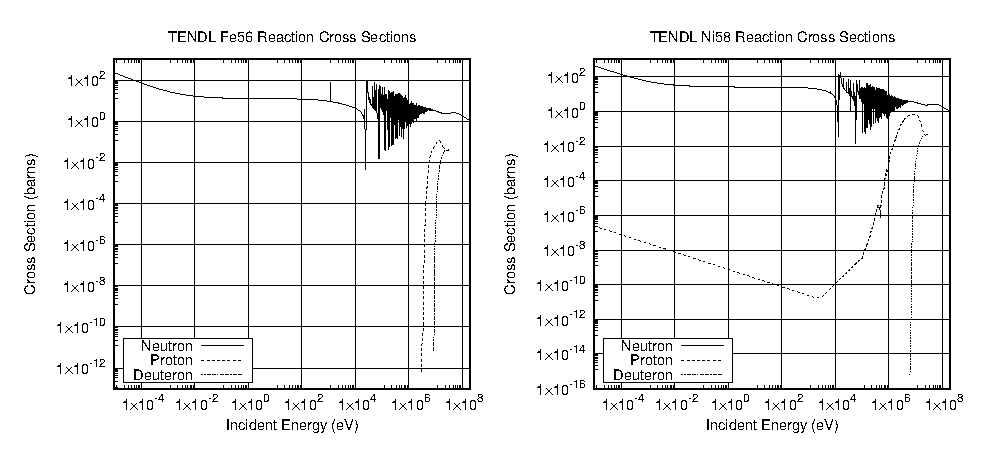
\includegraphics[width=15.0cm]{chapters/background_activity/plots/npd_xs/fe56_ni58_xs.eps}
    \captionsetup{font={it}}
    \caption{Electricity in Millions of Tonnes of Oil Equivalent}
    \label{fig:electricityusagesuk}
  \end{center}
\end{figure}







\subsection{Transmutation of Nuclei by Neutrons and Protons}

\subsubsection{Neutron Activation}

The fission of Uranium-235 atoms results in neutrons with a varied spectrum of energies.  The neutrons will bounce around inside the reactor losing energy quickly to light atoms within 



\subsubsection{Proton Activation}

Considering a simplified nuclear potential well, energetic protons approaching a nucleus may overcome the Coulomb potential barrier.  They are captured by the nucleus and held within the potential well by the strong nuclear force.  This process may leave the nucleus in an excited and unstable state, depending on the input energy of the proton and configuration of nucleons.  The process is probabilistic, and the average chance of a reaction (the microscopic cross section) may be measured as a function of the projectile, projectile energy and target, either experimentally or by optical model potential calculations.  The reaction rate is calculated from the microscopic cross section using the following equation:

\begin{equation}
R = \frac{J}{e} n_{t} \sigma \cdot 10^{-28} \delta t
\end{equation}

\begin{itemize}
\item R	Reaction Rate (reactions per second)
\item J	Beam current (A)
\item \ensuremath{n_t}	Number density of target (atoms per cubic metre)
\item \ensuremath{\sigma}	Microscopic reaction cross section (barns)
\item e	Elementary charge (1.602177E-19C)
\item \ensuremath{\delta}T	Target thickness (m)
\end{itemize}



\subsection{Nuclear Reaction Cross Sections}

\subsubsection{Reaction Cross Sections}






\subsubsection{TENDL Data Files}

The cross section data for protons and neutrons is available to download in ENDF format files.  The data files used by this work are TENDL data files, and these are created by a combination of different nuclear models and experimental data.  The TALYS nuclear reaction simulation code provides the calculated data.

The nuclear raction files are rather large, and they all follow, reasonably well, a standard format.

Each reaction file is itself (confusingly, to begin with) split into multiple "files".  




\subsubsection{TALYS Models}






\subsubsection{Relative Amounts of Isotopes}



\begin{equation}
p_{m,k} = 100 \times \frac{p_{n,k} \times A_{k}}{\sum_{i=1,N}(p_{n,i} \times A_i}
\end{equation}




\begin{equation}
p_{n,k} = 100 \times \frac{\frac{p_{m,k}}{A_{k}}}{\sum_{i=1,N}(\frac{p_{m,i}}{A_i})}
\end{equation}







\subsection{Radioactive Decay}

Radioactive decay is the random change in nucleons or energy state of an unstable nucleus.  It is impossible to predict when a single nucleus will decay, but the decay of a collection of nuclei is statistical in nature.  The radioactivity and number of unstable nuclei at time t can be predicted using the decay constant, \textlambda, for the radioactive isotope.  This constant is defined as follows:

\begin{equation}
\lambda = - \frac{N'(t)}{N(t)}
\end{equation}

The number of radioactive nuclei N(t) at time t is given by the following equation, where N(0) is the starting number of nuclei:

\begin{equation}
N(t) = N(0) \exp(-t \lambda)
\end{equation}

The activity A(t) of the radioactive nuclei is predicted at time t by using the following equations, where N'(t) is the change in amount of nuclei with respect to time:

\begin{equation}
A(t) = -N'(t) = \lambda N(t)
\end{equation}
\begin{equation}
A(t) = \lambda N(0) \exp(-t \lambda)
\end{equation}

\subsection{Bateman Equation for Radioactive Decay}

%% Define tikz boxes
\tikzstyle{startstop} = [rectangle, rounded corners, minimum width=3cm, minimum height=1cm,text centered, draw=black, fill=grey!30]
\tikzstyle{process} = [rectangle, minimum width=3cm, minimum height=1cm, text centered, draw=black, fill=grey!10]
\tikzstyle{arrow} = [thick,->]

\begin{figure}[!h]
\centering
\begin{tikzpicture}[node distance=2cm]
\node (parent) [startstop] {Parent Isotope, N$_{\text{1}}$(t)};
\node (isotope1) [process, below of=parent] {1st Unstable Daughter Isotope, N$_{\text{2}}$(t)};
\node (isotope2) [process, below of=isotope1] {2nd Unstable Daughter Isotope, N$_{\text{3}}$(t)};
\node (stable) [startstop, below of=isotope2] {Stable Daughter Isotope, N$_{\text{4}}$(t)};
%% arrows
\draw [->] (parent) -- (isotope1);
\draw [->] (isotope1) -- (isotope2);
\draw [->] (isotope2) -- (stable);
\end{tikzpicture}
\captionsetup{font={it}}
\caption{An example decay chain from an unstable parent isotope, through unstable daughter isotopes ending with a stable daughter isotope.}
\label{fig:decaychain}
\end{figure}

The English mathematician Harry Bateman derived an equation (\ref{eq:bateman}) to calculate the amount of each isotope in a decay chain, illustrated in Figure \ref{fig:decaychain}, at time t.

\begin{equation}
N_{n}(t) = \sum_{i=1}^{i=n} \left( \left( \prod_{j=i}^{j=n-1} \lambda_{(ij+1)}\right) \sum_{j=i}^{j=n} \left(\frac{N_{i0}\exp(-\lambda_{j}t)}{\prod_{p=i,p\neq j}^{p=n} (\lambda_{p} - \lambda_{j})}\right)\right)
\label{eq:bateman}
\end{equation}

When a radioactive isotope decays, there may be more than one mode of decay, and this leads to branching factors.  Pb-214 only decays via beta decay to Bi-214, giving a branching factor of 1.0, whereas Bi-214 has a 99.979\% chance of decaying to Po-214 by beta decay and a 0.021\% of emitting an alpha particle and decaying to Tl-210 (branching factors of 0.99979 and 0.00021 respectively) \cite{jeff311}.

When a target material is irradiated, there is a source term for transmuted nuclei due to the irradiation.  The daughter isotopes of these transmuted isotopes will also be affected by the irradiation and will transmute further, giving a source term for each daughter isotope as a result of the irradiation.  Sources for each isotope in the decay chain, and branching factors between a parent isotope and its daughter isotope/s must be accounted for.




















\subsection{Simulating Ion Irradiation with SRIM}

Move to Method

A package of ion transport codes, SRIM, is freely available to download and use to investigate the transport of ions through matter.  SRIM uses the binary collision approximation (BCA) to simulate the passage of ions in a material.  It is an approximate method, and one key restriction is that it does not take into account the structure of the material, and this approximation is therefore also imposed on the Activity code.

\begin{figure}
  \begin{center}
    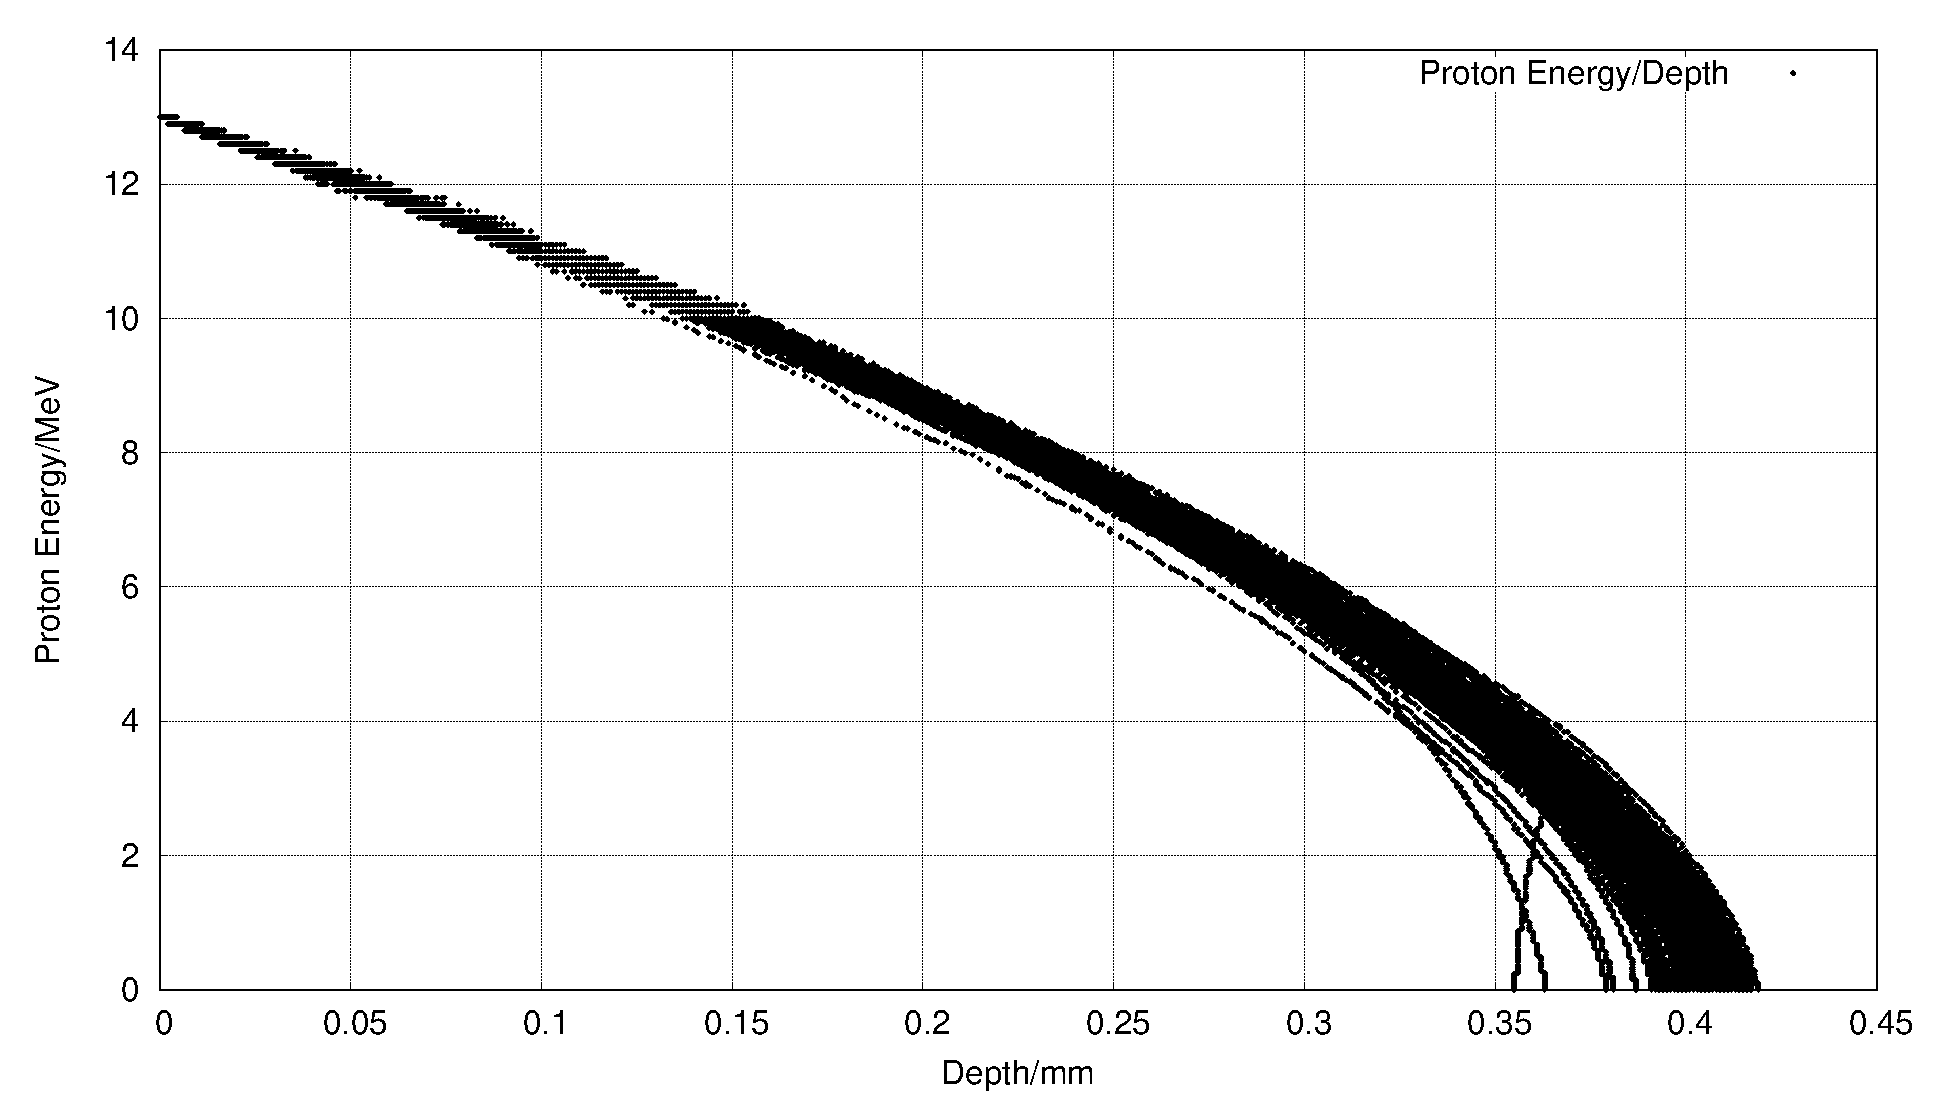
\includegraphics[width=15.0cm]{chapters/background_activity/plots/fe_13MeV.eps}
    \captionsetup{font={it}}
    \caption{One hundred simulated 13MeV proton energy loss curves in Fe simulated with SRIM \cite{srim}}
    \label{fig:fe13traj}
  \end{center}
\end{figure}

One file that SRIM creates is of importance to the Activity code, and that is the trajectory file that contains the energy and x,y,z co-ordinate data points for simulated ions moving through matter.  Figure \ref{fig:fe13traj} shows the trajectory of one hundred 13MeV protons entering and passing through an Iron target, and it is this set of data points (together with the cross section database) that the Activity code uses to calculte the reaction rates for the transmutation of nuclei in the target.  At higher energies, the ions slow as they lose energy due to electronic stopping, but as the ion energy drops the mechanism of loss through nuclear collisions becomes important.  The spreading of ion depths at lower energies is a result of the higher momentum transfer during nuclear collisions, as can be seen in Figure \ref{fig:fe13traj}.